\documentclass[a4paper,12pt]{article}

\usepackage[T2A]{fontenc}
\usepackage[utf8]{inputenc}
\usepackage[russian]{babel}
\usepackage{hyperref}
\usepackage{graphicx}
\usepackage{tcolorbox}
\usepackage{enumitem}
\usepackage{listings}
\usepackage{xcolor}
\usepackage{geometry}
\usepackage{placeins}

\geometry{
    a4paper,
    total={170mm,257mm},
    left=20mm,
    right=20mm,
    top=20mm,
    bottom=20mm,
}

\hypersetup{
    colorlinks=true,
    linkcolor=blue,
    filecolor=magenta,      
    urlcolor=cyan,
    pdftitle={Инструкция по работе с AI-ассистентом куратора проектного практикума},
    pdfpagemode=FullScreen,
}

\lstset{
    basicstyle=\ttfamily\small,
    breaklines=true,
    frame=single,
    numbers=left,
    numberstyle=\tiny\color{gray},
    keywordstyle=\color{blue},
    commentstyle=\color{green!60!black},
    stringstyle=\color{red},
    backgroundcolor=\color{gray!10},
}

\title{Инструкция по работе с AI-ассистентом куратора проектного практикума}
\author{}
\date{}

\begin{document}

\maketitle
\tableofcontents
\newpage

\section{Назначение приложения}
AI-ассистент куратора проектного практикума - это инструмент, который помогает автоматизировать проверку отчетов студенческих проектов, используя технологии искусственного интеллекта. Он анализирует содержание документов, оценивает их по заданным критериям и формирует структурированную обратную связь.

\section{Обзор интерфейса}

\begin{samepage}
Приложение содержит три вкладки:
\begin{itemize}
    \item \textbf{Проверка проектов} (основная вкладка)
    \item \textbf{Управление промптами} - для просмотра и редактирования текстов запросов к языковым моделям
    \item \textbf{О проекте} - информация с описанием приложения
\end{itemize}
\end{samepage}

\begin{figure}[!htb]
    \centering
    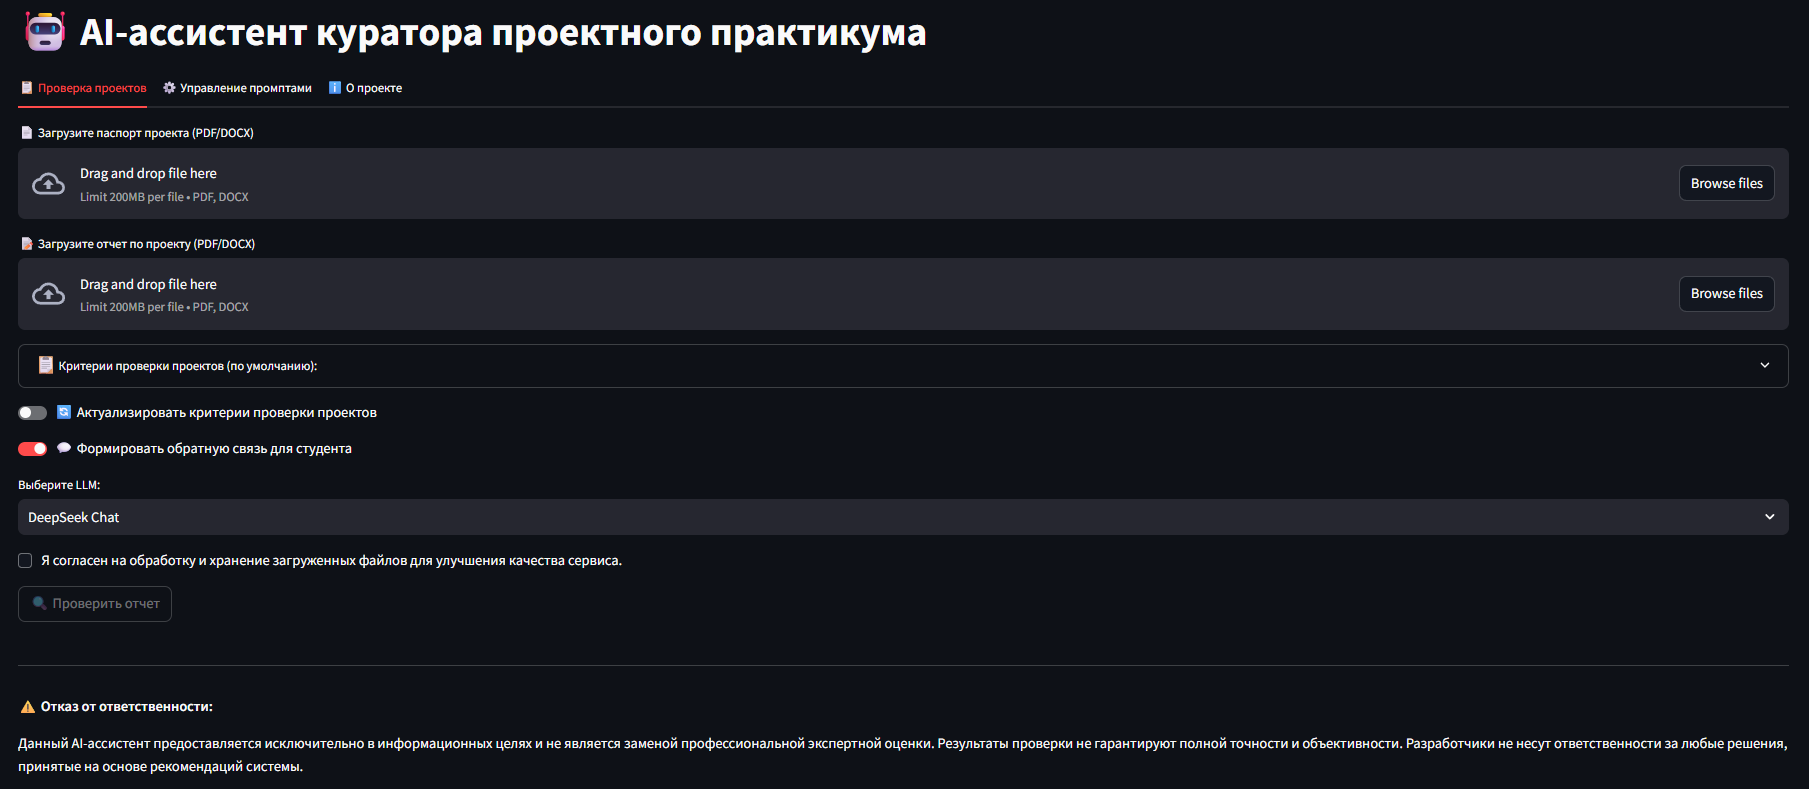
\includegraphics[width=\linewidth]{assets/interface.png}
    \caption{Общий вид интерфейса приложения}
\end{figure}

\FloatBarrier
\section{Работа с приложением}

\subsection{Вкладка ``Проверка проектов''}

\begin{samepage}
\subsubsection{Загрузка файлов}
\begin{itemize}
    \item \textbf{Паспорт проекта} (необязательный файл в формате PDF или DOCX)\\
    \textit{Содержит описание предметной области проекта и требования к конечному результату.\\
    Необходим для адаптации критериев под тематику проекта.}
    
    \item \textbf{Отчет по проекту} (обязательный файл в формате PDF или DOCX)\\
    \textit{Документ, который будет анализироваться и оцениваться системой.}
\end{itemize}
\end{samepage}

\begin{tcolorbox}[colback=blue!5!white,colframe=blue!75!black,title=Совет]
Для наилучших результатов рекомендуется загружать оба документа. Это позволит системе лучше понять контекст проекта и выполнить адаптацию критериев.
\end{tcolorbox}

\begin{figure}[!htb]
    \centering
    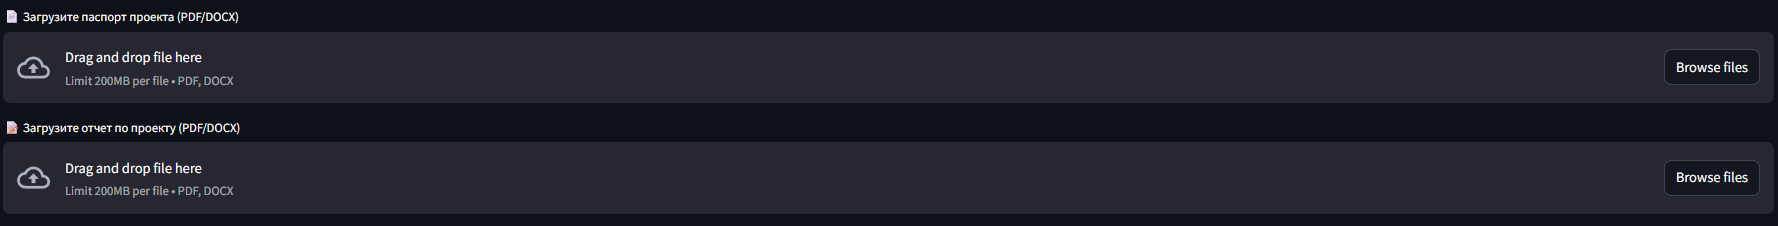
\includegraphics[width=\linewidth]{assets/upload_files.png}
    \caption{Секция загрузки файлов}
\end{figure}

\FloatBarrier
\begin{samepage}
\subsubsection{Критерии проверки}
\begin{itemize}
    \item \textbf{Стандартные критерии} (используются по умолчанию):
    \begin{itemize}
        \item Содержат критерии для различных типов проектов (прикладных и исследовательских)
        \item Доступны для просмотра через выпадающую секцию ``Критерии проверки проектов (по умолчанию):''
    \end{itemize}

    \item \textbf{Пользовательские критерии} (опционально):
    \begin{itemize}
        \item Активируйте переключатель ``Актуализировать критерии проверки проектов''
        \item Загрузите файл с критериями (поддерживаемые форматы: TXT, PDF, DOCX)
    \end{itemize}
\end{itemize}
\end{samepage}

\begin{tcolorbox}[colback=blue!5!white,colframe=blue!75!black,title=Примечание]
Если загружен паспорт проекта, система автоматически адаптирует критерии под тематику и требования проекта.
\end{tcolorbox}

\begin{figure}[!htb]
    \centering
    
\includegraphics[width=\linewidth]{assets/criteria.png}
    \caption{Секция критериев проверки}
\end{figure}

\FloatBarrier
\begin{samepage}
\subsubsection{Дополнительные настройки}
\begin{itemize}
    \item \textbf{Формировать обратную связь для студента}\\
    \textit{Если включено, система создаст структурированный текст с рекомендациями для студента}
    
    \item \textbf{Выбор модели для выполнения проверки}\\
    Доступные модели:
    \begin{itemize}
        \item DeepSeek Chat
        \item DeepSeek R1
        \item YandexGPT Pro 
        \item YandexGPT Lite
        \item Gemini 2.0 Flash
        \item Qwen 32B
        \item Qwen 2.5 72B
    \end{itemize}
\end{itemize}
\end{samepage}

\begin{tcolorbox}[colback=blue!5!white,colframe=blue!75!black,title=Совет]
Если результаты проверки вас не устраивают, попробуйте использовать другую модель.
\end{tcolorbox}

\begin{figure}[!htb]
    \centering
    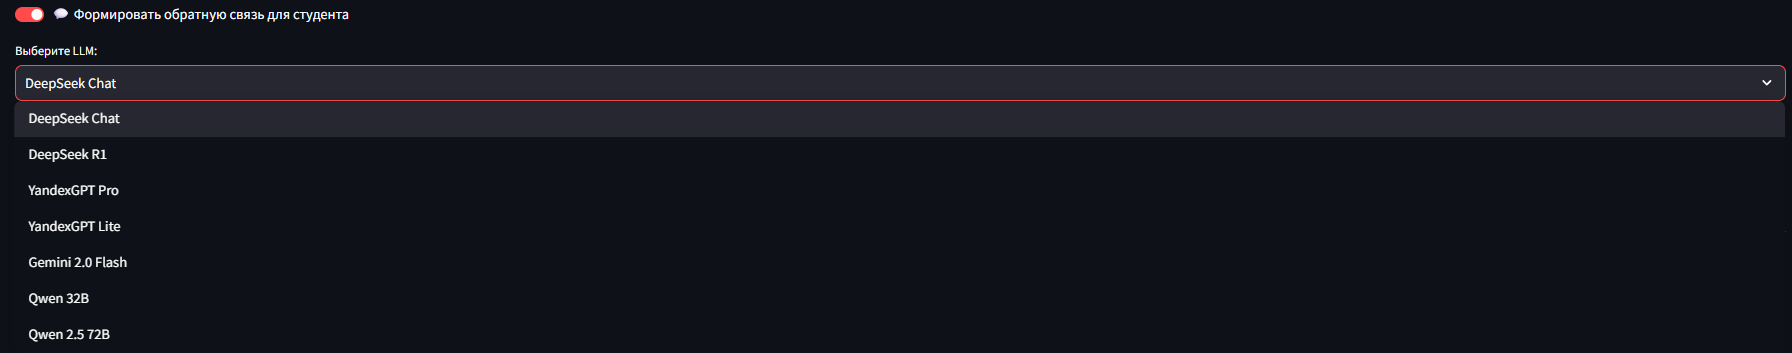
\includegraphics[width=\linewidth]{assets/additional_settings.png}
    \caption{Секция дополнительных настроек}
\end{figure}

\FloatBarrier
\begin{samepage}
\subsubsection{Запуск проверки}
\begin{enumerate}
    \item Установите флажок согласия на обработку и хранение файлов.
    
    \item Нажмите кнопку ``Проверить отчет''
    
    \item Дождитесь завершения процесса проверки 
    \begin{itemize}
        \item Во время проверки будет отображаться текущий этап выполнения
        \item Не закрывайте вкладку браузера до завершения проверки
    \end{itemize}
\end{enumerate}
\end{samepage}

\begin{figure}[!htb]
    \centering
    
\includegraphics[width=\linewidth]{assets/check_start.png}
    \caption{Запуск процесса проверки}
\end{figure}

\FloatBarrier
\begin{samepage}
\subsubsection{Результаты проверки}
После завершения проверки отображаются три раздела (можно развернуть каждый, нажав на заголовок):

\begin{itemize}
    \item \textbf{Адаптированные критерии проверки}
    \begin{itemize}
        \item Критерии, которые были использованы для проверки
        \item Если был загружен паспорт, критерии учитывают его требования
    \end{itemize}

    \item \textbf{Результаты проверки}
    \begin{itemize}
        \item Детальный анализ соответствия отчета каждому критерию
    \end{itemize}

    \item \textbf{Обратная связь для студента} (если опция была включена)
    \begin{itemize}
        \item Готовый структурированный текст с конструктивными замечаниями и рекомендациями
        \item Можно скопировать и использовать как основу для обратной связи
    \end{itemize}
\end{itemize}
\end{samepage}

\begin{figure}[!htb]
    \centering
    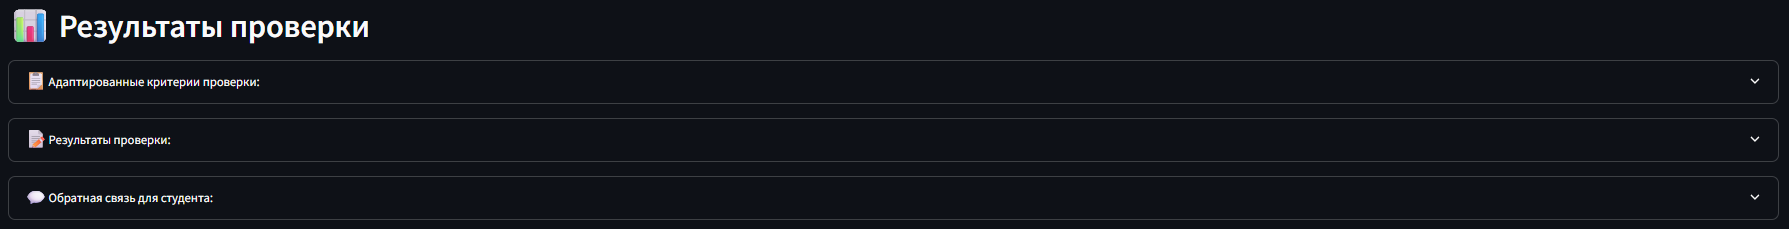
\includegraphics[width=\linewidth]{assets/check_results.png}
    \caption{Результаты проверки}
\end{figure}

\FloatBarrier
\begin{samepage}
\subsubsection{Сохранение результатов}
Вы можете сохранить результаты проверки для дальнейшего использования:

\begin{enumerate}
    \item Выберите предпочтительный формат файла из выпадающего списка:
    \begin{itemize}
        \item \textbf{HTML} (по умолчанию) - открывается в браузере, сохраняет форматирование
        \item \textbf{PDF} - формат для печати и официальных документов
        \item \textbf{Markdown} - текстовый формат с разметкой, удобен для дальнейшего редактирования
    \end{itemize}

    \item Нажмите кнопку ``Скачать результаты (выбранный формат)''
\end{enumerate}
\end{samepage}

\begin{figure}[!htb]
    \centering
    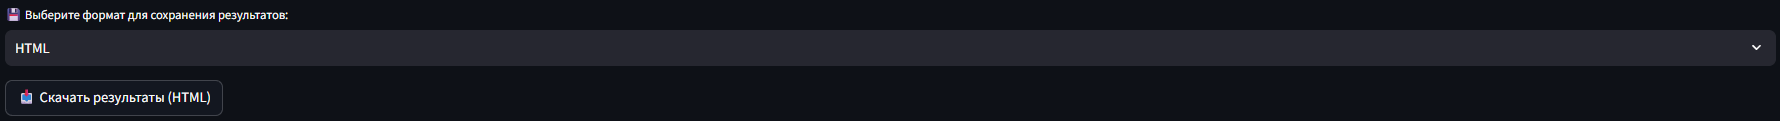
\includegraphics[width=\linewidth]{assets/save_results.png}
    \caption{Секция сохранения результатов}
\end{figure}

\FloatBarrier
\begin{samepage}
\subsubsection{Обратная связь о качестве проверки}
Ваше мнение поможет улучшить работу сервиса:

\begin{enumerate}
    \item Откройте раздел ``Оставить обратную связь о результатах проверки''
    \item Оцените качество проверки (хорошо или плохо).
    \item Добавьте комментарий (необязательно), указав:
    \begin{itemize}
        \item Что было особенно полезным
        \item Предложения по развитию сервиса
    \end{itemize}
    \item Нажмите ``Отправить обратную связь''
\end{enumerate}
\end{samepage}

\begin{figure}[!htb]
    \centering
    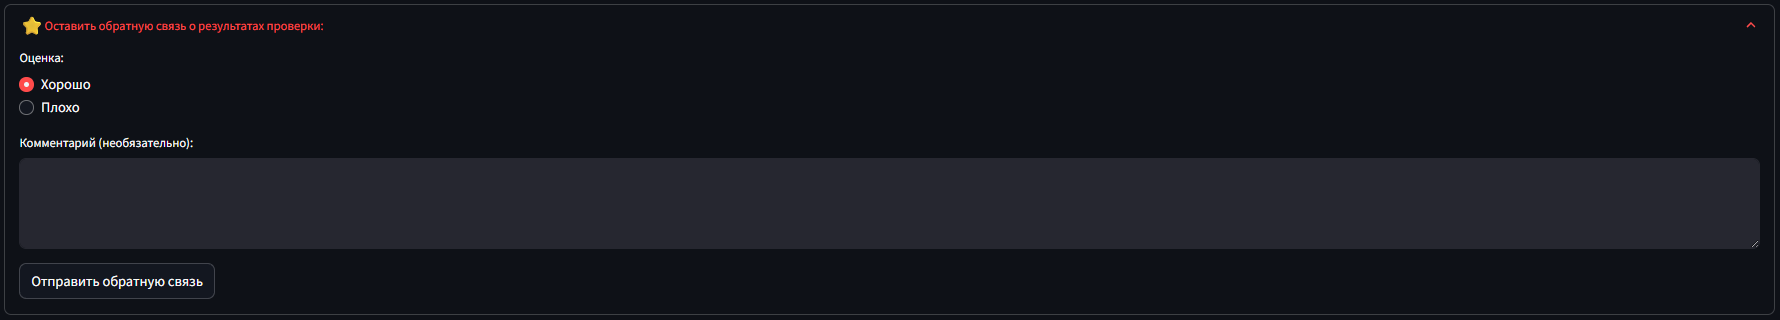
\includegraphics[width=\linewidth]{assets/feedback_form.png}
    \caption{Форма обратной связи}
\end{figure}

\FloatBarrier
\begin{samepage}
\subsection{Вкладка ``Управление промптами''}
В этой вкладке вы можете просматривать и редактировать шаблоны запросов к языковым моделям:

\begin{itemize}
    \item \textbf{Формирование критериев} (CRITERIA\_FORMING\_TEMPLATE) - шаблон для адаптации критериев под тематику и требования проекта
    \item \textbf{Проверка отчета} (CHECK\_REPORT\_TEMPLATE) - шаблон для проверки отчета в соответствии с критериями
    \item \textbf{Формирование обратной связи} (FEEDBACK\_FORMING\_TEMPLATE) - шаблон для формирования обратной связи студенту
\end{itemize}

Интерфейс управления промптами включает:
\begin{enumerate}
    \item Выпадающий список для выбора типа промпта
    \item Текстовое поле для просмотра и редактирования содержимого
    \item Кнопки управления:
    \begin{itemize}
        \item ``Сохранить изменения'' - для сохранения внесенных правок
        \item ``Сбросить этот промпт'' - для сброса текущего промпта к стандартному шаблону
        \item ``Сбросить все промпты'' - для сброса всех промптов к стандартным шаблонам
    \end{itemize}
\end{enumerate}
\end{samepage}

\begin{tcolorbox}[colback=red!5!white,colframe=red!75!black,title=Важно]
При редактировании не изменяйте и не удаляйте переменные в формате \{...\}. Они используются для подстановки данных при выполнении проверки. 
\end{tcolorbox}

\begin{figure}[!htb]
    \centering
    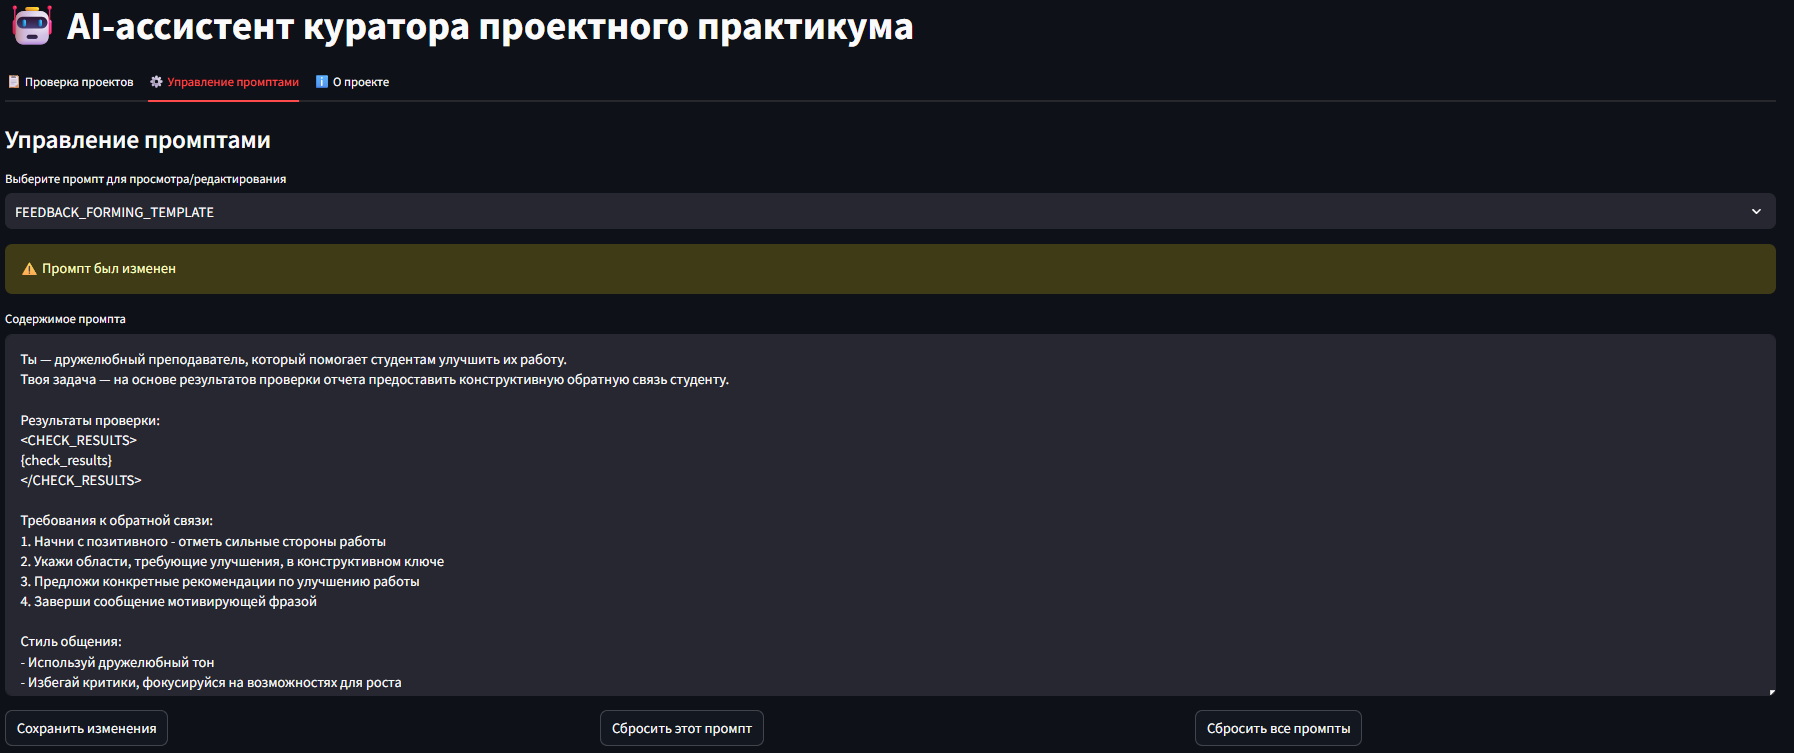
\includegraphics[width=\linewidth]{assets/prompt_management.png}
    \caption{Интерфейс управления промптами}
\end{figure}

\FloatBarrier
\begin{samepage}
\subsection{Вкладка ``О проекте''}
Содержит подробную информацию о проекте:

\begin{itemize}
    \item Назначение и цели AI-ассистента
    \item Описание функциональных возможностей
    \item Используемые технологии
\end{itemize}
\end{samepage}

\begin{figure}[!htb]
    \centering
    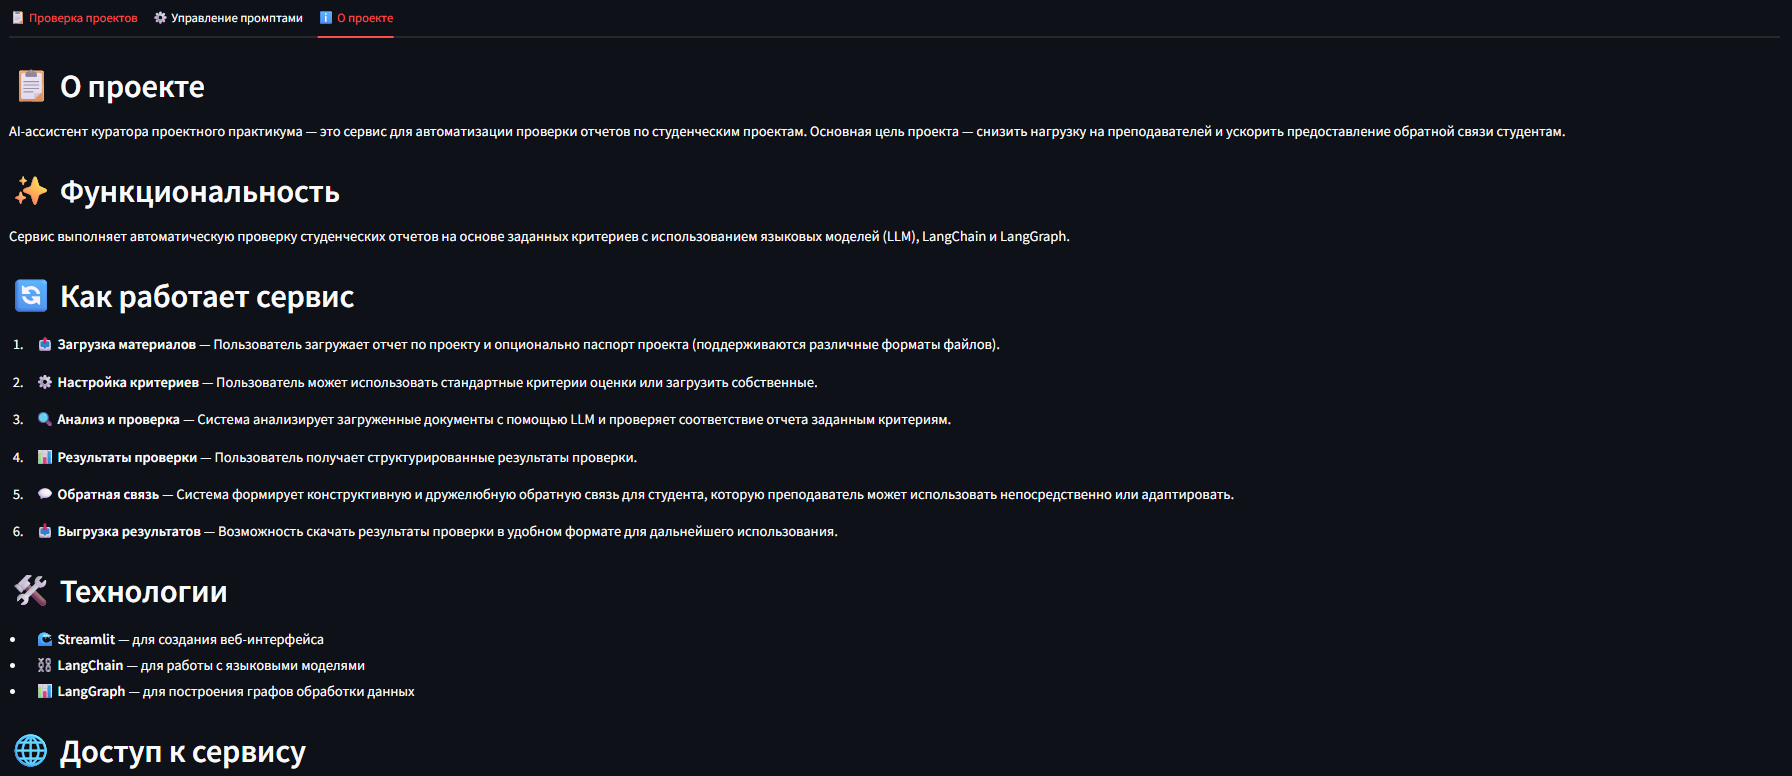
\includegraphics[width=\linewidth]{assets/project_info.png}
    \caption{Информация о проекте}
\end{figure}

\end{document} 